
\chapter{Cache Management Algorithms}
\label{cpt:algorithms}


A cache management algorithm manages the storage space in a cache.
It decides where to store new data blocks and which of the existing blocks are evicted to make room for new blocks.
Some algorithms are thread-aware and geared towards shared caches.
Others are thread-agnostic and work both for shared and private caches.
Some have advanced optimization goals such as quality of service (QoS) while others use simpler metrics like miss minimization.
Algorithms proposed for shared caches may in general be divided into two groups, those that explicitly divide storage space between cores sharing the cache and those that do not.
The term cache replacement algorithm is often used to describe algorithms that do not divide the storage space while the term cache partitioning algorithm describe algorithms that do divide the space.
Throughout this paper, we will use the two terms interchangeably.

The field of cache management is well researched, and there exists a large number of proposed algorithms.
In this thesis, we present a few recently proposed algorithms and compare their performance.
We will also present LRU, an algorithm that is thread-agnostic and widely used both in private and shared caches today.
Table~\ref{tbl:algorithms} lists the selected algorithms.
Only algorithms that optimize for fewer cache misses are included.
This metric is easy to measure and also makes it easy to compare the various algorithms.
Also, we only consider algorithms that target conventional caches, as they are designed in CMPs today.
This limitation makes the comparison of results from different algorithms easier.
Also, we avoid having to extend our simulator with a new cache type, which would be unfeasible given the time constraints of this thesis.

\begin{table}[thb]
\begin{tabular}{|p{1.4cm}|p{0.5cm}|p{0.8cm}|p{1.2cm}|p{1.2cm}|p{1.4cm}|p{1.2cm}|p{1.0cm}|}
\hline
\multicolumn{1}{|c|}{Name} & \multicolumn{1}{c|}{Year} & \multicolumn{1}{c|}{Thread} & \multicolumn{1}{c|}{Repl.} & \multicolumn{1}{c|}{Insert.} & \multicolumn{1}{c|}{Promo.} & \multicolumn{1}{c|}{Hardware}    & \multicolumn{1}{c|}{Partition}     \\
\multicolumn{1}{|c|}{}          & \multicolumn{1}{c|}{}          & \multicolumn{1}{c|}{aware}  & \multicolumn{1}{c|}{policy}      & \multicolumn{1}{c|}{policy}    & \multicolumn{1}{c|}{policy}    & \multicolumn{1}{c|}{overhead\footnotemark}  & \multicolumn{1}{c|}{}       \\ \hline
DIP                             & 2007                           & No                          & LRU                              & LIP/ BIP                        & Promote to MRU            & 1 counter, set dueling    & No            \\ \hline
TADIP                           & 2008                          & Yes                         & LRU                              & LIP/ BIP                        & Promote to MRU            & 1 counter per core, set dueling  & No          \\ \hline
DRRIP                           & 2010                          & Yes                         & LRU approx.                      & SRRIP/ BRRIP                    & Stepwise promotion            & 1 counter per core, set dueling  & No          \\ \hline
NUCache                         & 2011                         & No                          & LRU + DeliWays     & LIP                            & Promote to MRU                 & NUTrack                            & No    \\ \hline
UCP                             & 2006                           & Yes                         & Per core LRU                     & LIP                            & Promote to MRU                 & UMON, 1 ATD per core   & Yes                \\ \hline
PIPP                            & 2009                           & Yes                         & LRU                              & Utility position               & Stepwise promotion            & UMON, 1 ATD per core, random generator & Yes \\ \hline
PriSM                           & 2012                           & Yes                         & Per core LRU                  & LIP                            & Promote to MRU                 & 1 ATD per core, random generator                       & Yes  \\ \hline
CLU                             & 2014                           & Yes                         & LRU                              & LIP/ BIP                        & Promote to MRU/ Skip            & UMON \~3 ATDs per core                & Yes  \\ \hline
\end{tabular}
\caption{Overview of Cache Management Algorithms.}
\label{tbl:algorithms}
\end{table}
\clearpage

It is possible to divide all algorithms included in this evaluation into three distinct policies:
\begin{itemize}
\item The replacement policy specifies which block a cache set evicts when inserting a new block into that set.
\item The insertion policy specifies the state of new blocks after insertion into the cache set.
\item The promotion policy specifies how the state of a block changes following an access from a processor core.
\end{itemize}
In the following sections, we will explain how each of the selected cache partitioning algorithms work, with an emphasis on this division to make comparisons easier.

\section{Cache Replacement Algorithms}
This section covers cache replacement algorithms, or algorithms that do not explicitly divide the available cache space between cores.


\footnotetext{Simplified hardware overhead compared to a LRU managed cached.}


\subsection{LRU}
\label{sec:algorithms:lru}

\begin{figure}[t]
    \centering
    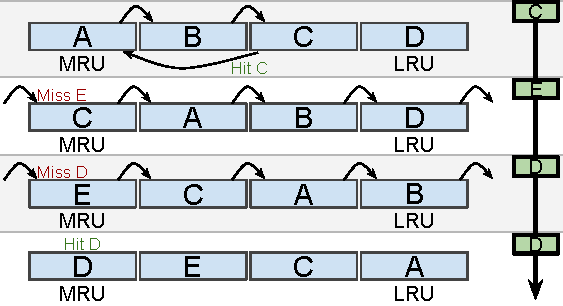
\includegraphics[width=.65\textwidth]{figures/algorithms/LRU}
    \caption{LRU managed 4-way cache set.}
    \label{fig:algorithms:lru_example}
\end{figure}

\noindent
\gls{lru} replacement, or some simplification of \gls{lru}, is one of the dominant cache management algorithms in hardware today. 
As a result, \gls{lru} is normally used as the baseline for comparisons when presenting new cache management algorithms~\cite{Jaleel2010,Qureshi2006,Qureshi2007}.

The \gls{lru} algorithm relies on the temporal locality of data accesses; it assumes that recently accessed data has a higher reuse frequency than less recently accessed data.
Theoretically one can envision a cache set managed by \gls{lru} as a stack, where recently accessed cache blocks are near the top and less recently accessed blocks are near the bottom.
The bottom position of the stack is the \gls{lru} position, and the top position is the \gls{mru} position.
In a hardware implementation, the blocks are not stored in a sorted fashion, but additional storage bits are used to keep track of \gls{lru} positions.
The replacement policy of \gls{lru} is to evict the least recently used cache block, the one on the bottom of the \gls{lru} stack.
The insertion and promotion policy of \gls{lru} is the same; a inserted or accessed block is always moved to the \gls{mru} position unless it is already there.

Figure~\ref{fig:algorithms:lru_example} shows how a 4-way cache set managed by \gls{lru} replacement handles four requests. 
Initially, the set contains four blocks; A, B, C and D. 
A is in the \gls{mru} position while D is in the \gls{lru} position.
The first request is for block C; this is a hit, and that causes the block to move to the \gls{mru} position, pushing both block A and B one step closer to the \gls{lru} position.
The second request is made to block E; this block is not present in the cache.
The \gls{lru} algorithm evicts block D at the \gls{lru} position and then places block E at the \gls{mru} position.
Then a request for D follows, this is a miss and B is evicted.
Finally, another request is made to block D. Nothing changes since the block already is at the \gls{mru} position.

One important result of the \gls{lru} insertion, promotion, and replacement policies is that an \gls{lru} managed cache satisfies the \textit{stack property}.
Given a 4-way \gls{lru} managed cache with counters that count the number of hits in each way; then we know that the number of misses in a 3-way \gls{lru} managed cache equals the misses in the 4-way cache plus the number of hits in the 4th cache way.
This effect occurs because any request that hits in the 4th way of the 4-way cache would miss in the 3-way cache, but in both caches the requested block is then moved to the \gls{mru} position.
No blocks can enter the cache set at any other position than the \gls{mru}.
As a result, the state of the three first ways of the caches is always identical given an identical memory request sequence.
The same argument holds for a 2-way cache, by summing the hits in the third and fourth way of the 4-way cache we get the additional misses in a 2-way cache.
This property generalizes; we can find the relative miss rate of any \gls{lru} managed cache with $1$ to $n$ ways by having a single n-way cache with access counters per way.
If we additionally have a total miss counter in the n-way cache we can also find the absolute number of misses for each cache size.

\gls{lru} is a simple replacement algorithm that is usable in both private and shared caches.
In shared caches, \gls{lru} will favor access frequency, giving cores that issue many cache requests more cache space than those who issue fewer requests. 
In some cases, this might be an acceptable solution. 
However, as we will discover, several thread-aware replacement algorithms claiming to outperform \gls{lru} exists. 

\section{DIP}
\label{sec:algorithms:dip}

\begin{figure}
    \centering
    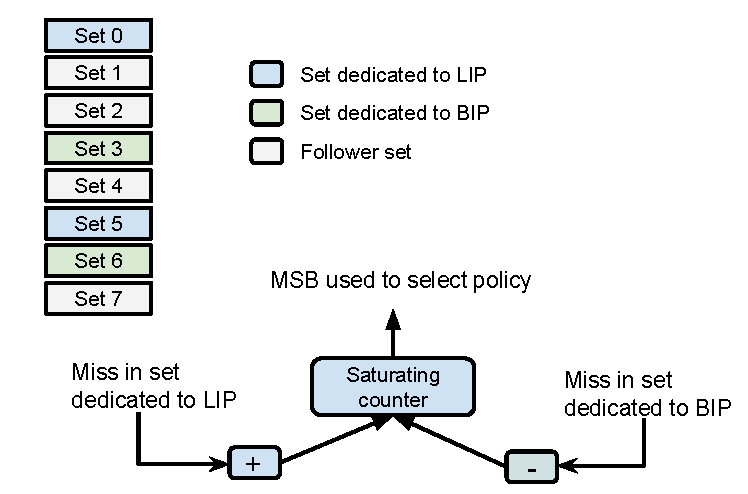
\includegraphics[width=\textwidth]{figures/algorithms/DIP_architecture}
    \caption{DIP set-dueling architecture}
    \label{fig:algorithms:dip:set_dueling}
\end{figure}

\begin{figure}
    \centering
    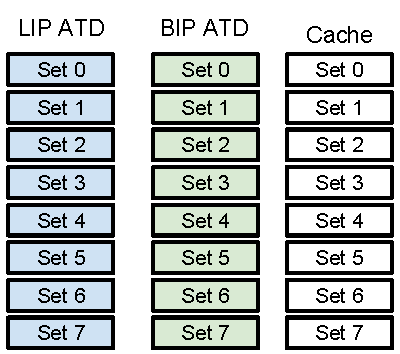
\includegraphics[width=\textwidth]{figures/algorithms/DIP_atd_architecture}
    \caption{DIP ATD architecture}
    \label{fig:algorithms:dip:atd}
\end{figure}

Dynamic Insertion Policy (DIP)~\cite{Qureshi2007} was originally proposed by M. K. Qureshi et al. in 2007.
The DIP algorithm views the cache set as a stack, as in LRU.
Replacement and promotion policies are equal to LRU, DIP evicts the block at the LRU position, and following a cache hit a block moves to the MRU position.
In contrast to LRU, DIP is a combination of two insertion policies, the standard LRU insertion policy (LIP) and Binominal Insertion Policy (BIP).
LIP inserts new blocks at the MRU position.
BIP inserts new blocks either at the LRU position or with a small probability, $p = \frac{1}{32}$, at the MRU position. 
The overall DIP algorithm switches between the two insertion policies by always using the one that is expected to cause fewer cache misses.

By mostly inserting at the LRU position the BIP insertion policy can theoretically handle trashing memory access patterns.
BIP inserts most of the new blocks in the LRU position, and the upper part of the LRU stack can contain blocks that have been re-referenced.
In a trashing access pattern, this results in part of the working set residing in the upper part of the stack while the rest are inserted at the LRU position and evicted at the next miss.
By sometimes inserting at the MRU position BIP will give blocks not referenced by the next miss a chance to stay in the cache. 
Inserting at the MRU position will also force stale cache blocks in the upper part of the stack to move towards the LRU position.

The authors of DIP present several methods to detect the best replacement algorithm, one of them is set-dueling.
Set-dueling is implemented by having some sets of the cache always use BIP and some always use LIP.
A counter tracks the performance of the dueling sets.
Misses in LRU sets will increment the counter and misses in BIP sets will decrement the counter.
The MSB of the counter can then be used to select the optimal algorithm.
If the MSB is one, an overweight of misses in LRU sets are occurring, and BIP is the optimal algorithm. 
If the MSB is zero, then an overweight of BIP misses are occurring, and LRU is the optimal algorithm.
Figure~\ref{fig:algorithms:dip:set_dueling} shows the set dueling and algorithm selection architecture suggested by M. K. Qureshi et al.
In the figure sets 0 and 5 are dueling sets for LIP while 3 and 6 are dueling sets for BIP.
All other sets are follower sets, meaning that they utilize the algorithm indicated by the selection logic.

Another solution is to utilize two Auxilliary Tag Directories (ATDs), as shown in figure~\ref{fig:algorithms:dip:atd}.
An ATD is equal to the caches tag directory; it keeps track of blocks present but does not store any data.
ATDs are, for this reason, cheaper than a full cache, but still requires more storage than dual-sets that use the existing cache.
As the figure shows, the two ATDs run one algorithm each, all operations on the main cache execute in parallel on the ATDs as well.
The same counter architecture controlled by misses in either ATD is used to select the optimal algorithm for the main cache.
The main advantage of using an ATD is that all available information is used when selecting between BIP and LIP.
Also, the entire cache will always use the best algorithm, where in set-dueling a fraction of the sets will always run the non-optimal algorithm.
\subsection{TADIP}
\label{sec:algorithms:tadip}

\begin{figure}[t]
    \centering
    \begin{subfigure}[b]{0.45\textwidth}
        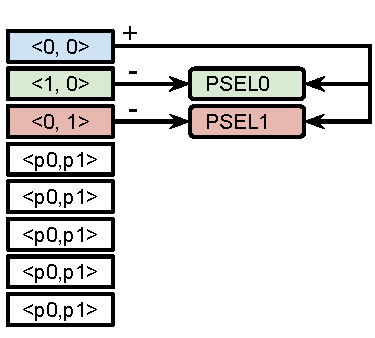
\includegraphics[width=\textwidth]{figures/algorithms/TADIP-I}
        \caption{Cache managed by \gls{tadip-i}.}
        \label{fig:algorithms:tadip:isolated}
    \end{subfigure}
    \begin{subfigure}[b]{0.45\textwidth}
        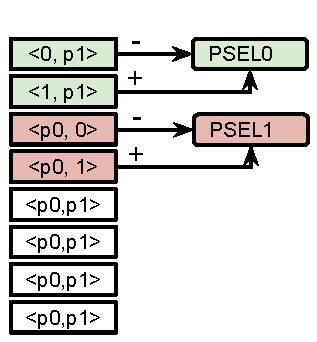
\includegraphics[width=\textwidth]{figures/algorithms/TADIP-F}
        \caption{Cache managed by \gls{tadip-f}.}
        \label{fig:algorithms:tadip:feedback}
    \end{subfigure}    
    \caption{Alternate duel set organizations for \gls{tadip}.}
    \label{fig:algorithms:tadip}
\end{figure}

\gls{tadip}~\cite{Jaleel2008} proposed in 2008 is a thread-aware extension of \gls{dip}~\cite{Qureshi2007}.
The main issue with \gls{dip} that \gls{tadip} counters, is that \gls{dip} does not consider which core initiates a cache access.
In a workload with multiple benchmarks, some might be recency-friendly while others are not. 
In a shared cache managed by \gls{dip}, the algorithm choice is made based on the sum of the cache accesses and then applied equally to all cores.
The authors of \gls{tadip} recognized that improvements in performance could be achieved by selecting the \gls{dip} policy on a per-core basis when utilized in a shared cache.

When selecting the best performing algorithm per core, the \gls{atd} technique requires two \glspl{atd} per core sharing the cache. 
This solution can quickly become too expensive to be practical.
Set-dueling in \gls{dip} requires a minimum of two sets, one running \gls{lip} (1) and one running \gls{bip} (0). 
With two cores, the number of combinations rises to four (00, 01, 10, 11).
When the number of cores increases this also seems to be an impractical solution.
Based on this observation, the authors of \gls{tadip} suggested two new selection techniques based on set dueling, which reduce the number of duel sets required.
Both solutions have one saturating counter per core sharing the cache.
This counter is used to select the best performing policy for that core.

\gls{tadip-i} has one set per core running \gls{bip} for that core and \gls{lip} for all others.
In addition to these N sets, a single set runs \gls{lip} for all cores. 
A miss in the \gls{lip} set will increment all the core counters while a miss in the core specific set will decrement the counter for the specific core.
For a large N, this solution requires significantly fewer duel sets compared to having one per combination ($N+1 << N^2$). 
This solution assumes that all other cores run \gls{lip}, and, therefore, cannot fully capture the effect of interactions between cores.
Figure~\ref{fig:algorithms:tadip:isolated} shows an example of a cache managed by \gls{tadip-i}. 
In the figure, PSEL0 is the saturating counter used to select the best performing policy for core 0.
Within a set; $<0, 0>$ indicates that both cores run \gls{lip} while $<1, 0>$ indicates that core 0 runs \gls{bip} while core 1 runs \gls{lip}.
The variables p0 and p1 represent the current best performing policy for core 0 and 1 respectively.

\gls{tadip-f} attempts to reduce the error caused by the assumption of other cores by having two sets per core, a total of 2N.
A cache managed by \gls{tadip-f} is illustrated in Figure~\ref{fig:algorithms:tadip:feedback}.
For each of the cores, one duel set use \gls{lip} and the other use \gls{bip}. 
Any insertions from other cores into the duel sets use the current best performing algorithm for that core.
Like in the other policies, a miss in the \gls{lip} set for a core will increment that core's counter and a miss the \gls{bip} set will decrement the counter.
For the remainder of this thesis when we refer to \gls{tadip} we assume \gls{tadip-f} unless otherwise stated.

When implementing \gls{tadip}, some mechanism is required to select which sets are duel sets, and which are follower sets.
The authors of \gls{tadip} provide a simple hash function that can be used to select dueling sets, shown in Algorithm~\ref{alg:algorithms:tadip:set_selection}.
This algorithm assumes a 4096 set cache.
In the algorithm, set index is a number from 0-4095, core\_id is the zero-indexed id of the requester core and cores is the total number of cores sharing the cache.
If \gls{bip} or \gls{lip} is true, then the set is a duel set for the given core, and the policy forced to either \gls{bip} or \gls{lip}.
If both \gls{bip} and \gls{lip} are false, then the set is a normal follower set and utilizes the current best performing algorithm for the given core.
It follows from the algorithms that the original authors use a total of 32 duel sets spread evenly throughout the cache.

\begin{algorithm}[ht]
\caption{TADIP duel set selection.}
\label{alg:algorithms:tadip:set_selection}
\begin{algorithmic}[1]
\State $LIP\gets set\_no[11:7] + core\_id == set\_no[6:0]$
\State $BIP\gets set\_no[11:7] + core\_id + cores == set\_no[6:0]$
\State $FOLLOWER\gets !LIP + !BIP$
\end{algorithmic}
\end{algorithm}

\subsection{DRRIP}
\label{sec:algorithms:drrip}

\begin{figure}[ht]
    \centering
    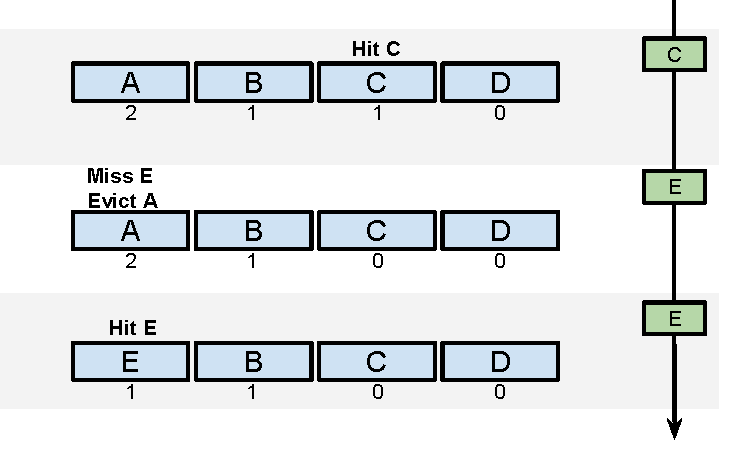
\includegraphics[width=.65\textwidth]{figures/algorithms/DRRIP}
    \caption[DRRIP managed 4-way cache set.]{DRRIP managed 4-way cache set. (M=2, static insertion)}
    \label{fig:algorithms:drrip_example}
\end{figure}

\gls{drrip}~\cite{Jaleel2010} was proposed in 2010.
\gls{drrip} does not utilize the concept of an \gls{lru} stack as done by \gls{lru} and \gls{tadip}.
In \gls{drrip}, each cache block has a number associated with it, called re-reference interval.
The re-reference interval is a relative measure of when the algorithm expects a block to be re-referenced.
Given two blocks with different re-reference intervals, then the block with a lower interval is expected to be re-referenced before the other block.
A value between 0 and $2^M - 1$ is used to represent the re-reference interval.
M is a configurable variable usually in the interval $[2, 5]$~\cite{Jaleel2010}.
The value of 0 indicates a \textit{near} re-reference interval, the algorithm expects the block to be re-referenced in the near future.
The value $2^M - 1$ indicates a \textit{distant} re-reference interval while the value of $2^M - 2$ indicates a \textit{long} re-reference interval.
Multiple blocks may have the same re-reference interval. 
Hence, blocks are not strictly ordered as in the \gls{lru} stack.
By setting $M=1$, \gls{drrip} degrades into the \gls{nru}~\cite{Microsystems2007} algorithm, which among others is used on the UltraSPARC T2.

The replacement policy of \gls{drrip} is to scan all blocks and evict the first one found with a distant re-reference interval.
If no blocks have a distant re-reference interval the re-reference interval of all blocks is incremented by one and the scan restarts.
This process repeats until the algorithm finds a victim block.
If multiple blocks are potential victims, the algorithm uses the scan order as a tie-breaker.
In the original paper, the authors specify that the leftmost potential block, the one with a lower block index, is the victim in the case of a tie.

\gls{drrip}'s promotion policy is to decrement the re-reference interval of the accessed block.
By doing this \gls{drrip} utilize access history rather than access time when calculating the re-reference interval.
Hence, to reach a near re-reference interval a block has to be accessed multiple times.
This promotion policy is different compared to \gls{lru} and \gls{tadip}, where a block will move to the \gls{mru} position following a hit, independent of the previous access history.

The insertion policy of \gls{drrip}, like \gls{dip} and \gls{tadip}, is composed of two different policies and a selection mechanism.
\gls{srrip} will always insert new blocks with a long re-reference interval. 
Depending on the state of the cache, there might be existing blocks with a higher re-reference interval than the blocks inserted by \gls{srrip}.
This gives the newly inserted blocks a chance to see a re-reference before being replaced.
\gls{brrip} is analog to \gls{bip} in \gls{dip}.
\gls{brrip} with either insert new blocks with a distant re-reference interval or, with a small probability, insert like \gls{srrip} with a long re-reference interval.
Like \gls{bip}, \gls{brrip} will allow trashing access patterns to keep some of the working set in the cache and hence improve performance over \gls{srrip}.
Selecting between the two insertion policies can be done using set dueling or \glspl{atd}, similar to what was described for \gls{tadip}.
The authors use set-dueling in their original paper, and we opt to do this in our implementation as well.

Figure~\ref{fig:algorithms:drrip_example} shows an example cache managed by \gls{drrip}.
In the example, M is set to 2, making the distant re-reference interval 3 and the long re-reference interval 2. 
Also, we assume static insertion throughout the example.
Initially, there are four blocks A, B, C and D with re-reference intervals 3, 1, 1 and 0.
First an access hits the C block, and its value decrements to 0.
Next a miss to block E occurs, block A has a re-reference interval of 3 and is evicted, E is assigned a re-reference interval of 2.
Then a miss to block D occurs, as no blocks have a re-reference interval of 3 all values are incremented by one.
After one incrementation E now has an interval of 3 and is evicted.
Then follows a hit to block D, causing its re-reference value to decrease by one.
The last row contains the final state of all blocks.

\subsection{NUCache}
\label{sec:algorithms:nucache}

\begin{figure}[ht]
    \centering
    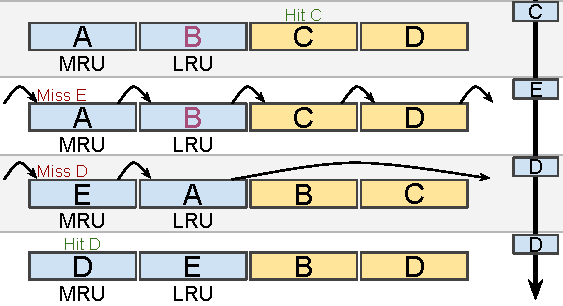
\includegraphics[width=.65\textwidth]{figures/algorithms/NUCache}
    \caption[NUCache managed 4-way cache set.]{NUCache managed 4-way cache set. (M=2)}
    \label{fig:algorithms:nucache_example}
\end{figure}

Next Use Cache (NUCache)~\cite{Manikantan2011} was first proposed in 2011.
NUCache does not partition the cache by examining each core's access pattern separately like many of the other algorithms. 
Instead, NUCache uses the concept of delinquent PCs.
A delinquent PC is the PC value of a memory instruction that often causes cache misses.
By evaluating the properties of the delinquent PCs, NUCache selects a set of PCs and allocates more cache space to blocks loaded by these instructions.
Because all applications running may contain one or more delinquent PCs, NUCache will implicitly share the cache between the applications.

To detect delinquent PCs, NUCache uses a novel DeliTrack structure.
The DeliTrack is a storage structure, indexed by PC that stores a miss count, insertion time and a next use histogram. 
\gls{lru} is used to manage the DeliTrack, which naturally ensures that PCs causing many misses are kept while others are replaced.
The next use histogram counts the next use value of blocks loaded into the cache by the given PC in buckets of 8 from 0 to 64.
This histogram is later used when a set of prioritized delinquent PCs are selected.

The next use distance of a block is defined as the number of misses observed by the cache between the time the block was evicted and the next time it is loaded due to a cache miss.
This number is then scaled by the number of sets in the cache to get the set relative next use distance.
An additional storage structure, NUTrack, is used to generate the next use histogram in the DeliTrack.
NUTrack is a set-associative structure indexed by block address.
Each row in the NUTrack stores a evicted bit, eviction time, and PC.
When a new block belonging to a PC in the DeliTrack is inserted into the cache, an attempt is made to insert a new row in the NUTrack. 
A row is inserted iff there is a valid replacement target in the NUTrack.
Two valid replacements exists; an unused row, or a row with the eviction bit set to true and an eviction time older than the maximum tracked next use value (64).
When a block is evicted from the main cache, the eviction bit and eviction time is set in the corresponding NUTrack row, if it exists.
On insertion in the main cache, the NUTrack searches for a matching row. 
If a matching row exists the next use distance is calculated and if the value is lower than the max value (64) the corresponding row in the DeliTrack histogram is incremented.

NUCache divides the ways in each cache set into two groups, MainWays, and DeliWays.
The MainWays are managed by \gls{lru} while the DeliWays are simply first in first out.
The value $M$ defines the number of DeliWays.
NUCache attempts to reduce misses by not evicting blocks from selected delinquent PCs when they are evicted from the MainWays, but rather let them enter the DeliWays.
By using the size of the DeliWays and the next use information in the DeliTrack structure, the algorithm periodically selects a set of PCs that are allowed to use the DeliWays.
The selection is done using a greedy algorithm that attempts to ensure that each block entering the DeliWays will receive a hit at least once before they are pushed out by other blocks.
DeliWays and MainWays are implemented by having two extra bits per cache block, one indicating if the block can enter the DeliWays, another indicating if the block is the DeliWays.
On insertion, all blocks inserted into to the MainWays.
When the \gls{lru} block in the MainWays is about to be replaced, the algorithm checks if it is marked to enter the DeliWays.
If the block is allowed to enter the DeliWays, it will not be evicted but rather moved from the MainWays.
If, after moving the new block into the DeliWays, the number of DeliWays blocks has exceeded $M$ the oldest block is removed.
Otherwise, the new \gls{lru} block in the MainWays is evaluated.
Because of this implementation the MainWays may use the entire cache if no DeliWays are in use, at the same time the DeliWays cannot exceed $M$.
This allows for an efficient use of every cache set.

Figure~\ref{fig:algorithms:nucache_example} shows an example cache set managed by NUCache with M set to 2.
Initially, there are four blocks, A, B, C, and D.
A and B are in the MainWays, indicated by the blue background.
While, C and D are in the DeliWays, as indicated by the yellow background.
Block B is eligible for insertion into the DeliWays, no other blocks in the example are eligible for the DeliWays.
The first request is for block C; this is a hit.
C is not promoted as it is a part of the FIFO managed DeliWays.
Next is a request for E, and this is a miss.
The cache first attempts to evict B, but B is eligible for DeliWays and is not evicted.
After B enters the DeliWays, it contains a total of 3 blocks, this is one more than the upper limit of 2, and hence the first in, D, is evicted.
E is then inserted at the MRU position.
Next is a request for D; this is also a miss, and A at the \gls{lru} position is evicted.
The final request is also for D, causing no change as D is already at the MRU position.



\section{Cache Partitioning Algorithms}
This section covers cache partitioning algorithms.
In contrast to the replacement algorithms, these algorithms explicitly assign a set number of blocks in each cache set to each core.

\subsection{UCP}
\label{sec:algorithms:ucp}

\gls{ucp}~\cite{Qureshi2006} was first presented in 2006. 
\gls{ucp} uses the concept of utility when assigning ways to a core.
Using a \gls{umon}, \gls{ucp} divides the ways in the cache between the cores.
\gls{ucp} then uses the same insertion and promotion policy as \gls{lru}.
The replacement policy is as in \gls{lru} but with two modifications:
First if the number of blocks owned by the requesting core is less than the number of ways assigned to it, then the least recently used block that is not assigned to the requester core is replaced.
If however the number of blocks owned is greater than or equal to the number of assigned ways the replacement algorithm selects the least recently used block of those owned by the requester.
This replacement policy ensures that the division between cores in each set move toward the global allocation following cache misses.
At the same time, a core may use more blocks that it is currently assigned, given that the space is not claimed by any other core.

The \gls{umon} is the core of the \gls{ucp} algorithm.
It consists of one \gls{atd} per core sharing the cache. 
The \gls{atd} is managed by normal \gls{lru} replacement and has one access counter per way.
Whenever a cache request hits in the \gls{atd}, the access counter representing the way the block was in is incremented.
In other words, \gls{umon} uses the stack property of \gls{lru}, as explained in Section~\ref{sec:algorithms:lru}, to find the hit rate of all valid partition sizes.
In addition to the \glspl{atd}, there is a monitor circuit that uses the access counters to calculate a new global partition at set intervals.
In the original paper, the authors recalculate the partitioning every 5M cycles.

The original paper proposes several algorithms for determining optimal partitioning based on the counter data. 
One of them is the Lookahead Algorithm suitable when there are more than two cores sharing a cache.
The Lookahead Algorithm assigns ways based on an increase in marginal utility; it is given in Algorithm~\ref{alg:algorithms:ucp}.
While there are more ways to distribute, the algorithm calculates the maximum marginal utility achievable by each core. 
The core with the highest value wins and is assigned as many ways as needed to achieve the increase.
The algorithm continue until all ways have been assigned.
Lines 27-28 calculate the marginal utility. 
First the number of misses prevented by increasing the allocation from a to b is found.
Due to the stack property of \gls{lru}, this is simply done by summing the access counters for ways $a$ to $b-1$.
The number of misses is then divided by the number of sets introduced, to find the marginal utility.
The rest of the algorithm is simply a greedy algorithm selecting the highest marginal utility at each iteration.
After a reallocation of cache ways, the \gls{atd} counters are all halved.
By doing this, the \gls{umon} will keep historical data for future decisions while prioritizing data from the current period.

Because the lookahead algorithm is greedy, finding a case where it makes a non-optimal choice is rather easy.
Consider a case with two cores, and two ways left to assign.
By assigning one way to core 0 it will receive 10 more hits, 2 ways offers no improvement.
Assigning one way to core 1 causes no additional hits, but if given two ways it will receive 18 hits.
In this case, the marginal utility is 10 for core 0 and 9 for core 1.
The algorithm assigns one way to core 0, and in the next iteration both have zero utility and it does not matter which is assigned the last way.
In this case, the algorithm saved 10 misses while it could have saved 18.
In order to guarantee optimal decisions the algorithm would have to do an exhaustive search of the solution space, but this is infeasible as it requires a lot more resources than the simplified greedy algorithm.

\begin{figure}[ht]
    \centering
    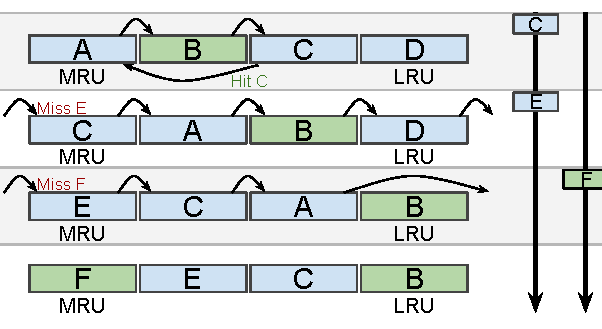
\includegraphics[width=.65\textwidth]{figures/algorithms/UCP}
    \caption[UCP managed 4-way cache set.]{UCP managed 4-way cache set. (Two cores each allocated two blocks)}
    \label{fig:algorithms:ucp_example}
\end{figure}

Figure~\ref{fig:algorithms:ucp_example} show an example cache set managed by \gls{ucp} shared by two cores.
We assume that both cores are allocated two blocks.
Initially, core 0 has three blocks in the cache as indicated by the blue background color; A, C, and D.
The first request is by core 0 for block C; this is a hit causing the block to be promoted to \gls{mru}, pushing A and B towards the \gls{lru} position.
Next is a request for E by core 0; this is a miss.
Because core 0 already has more than the number of allocated blocks in the cache, the block closest to \gls{lru} owned by core 0 is evicted, D in this case.
Finally, a request for F is made by core 1; this is also an miss.
Because core 1 has less than the number of allocated blocks in the cache, a block not owned by core 1 is to be evicted.
As a result, B owned by core 1 at the \gls{lru} position is saved, and rather A at the next to \gls{lru} position is evicted.



\begin{algorithm}[ht]
\caption{UMON Lookahead Algorithm.}
\label{alg:algorithms:ucp}
\begin{algorithmic}[1]
\State $balance\gets N$ /* Number of ways */
\State $allocations[i]\gets 0$ /* for each core $i$ */
\While {$balance$}
    \ForAll {$cores\ i$}
        \State $alloc\gets allocatations[i]$
        \State $max\_mu[i]\gets \Call{get\_max\_mu}{i, alloc, balance}$
        \State $blocks\_req[i]\gets$ min blocks to get max\_mu[i] for i
    \EndFor
    \State $winner\gets$ application with the maximum value of max\_mu
    \State $allocations[winner] += blocks\_req[winner]$
    \State $balance -= blocks\_req[winner]$
\EndWhile
\State \Return alloactions
\State

\Function{get\_max\_mu}{$i, alloc, balance$}
    \State $max\_mu\gets 0$
    \For{$ii = 1; ii <= balance; ii++$}
        \State $mu\gets \Call{get\_mu\_value}{p, alloc, alloc+ii}$
        \If{$mu \ge max\_mu$}
            \State $max\_mu\gets mu$
        \EndIf
    \EndFor
    \State \Return{$max\_mu$}
\EndFunction
\State

\Function{get\_mu\_value}{$p, a, b$}
    \State $U\gets$ change in misses for application p when number of blocks assigned to it increases from a to b
    \State \Return{$\frac{U}{b-a}$}
\EndFunction
\end{algorithmic}
\end{algorithm}

\subsection{PIPP}
\label{sec:algorithms:pipp}

Promotion/Insertion Pseduo-Partitioning~\cite{Xie2009} (PIPP) proposed in 2009 is an algorithm based on a slightly modified UMON circuit and a novel insertion and promotion policy.
The UMON changes are to enable stream detection.
Where the UCP algorithm only handles streaming applications indirectly, by assigning few ways because of a low hit rate in the ATDs, PIPP's UMON actively detects streaming applications.
Stream detection is implemented by adding a counter that counts the total number of cache misses in the ATD.
An application is then deemed to be streaming if either the number of misses or the miss rate in a single allocation period is above a threshold.

PIPP like UCP views the cache set as an LRU stack.
The replacement policy is as in LRU, but the insertion and promotion policy is novel.
The insertion policy inserts new blocks $\pi_n$ blocks from the LRU position. 
Here $\pi_n$ is the number of ways assigned to the $n^{th}$ core.
In a 4-way cache dual-core setup where both cores are assigned two ways, PIPP will insert all new blocks from either core in the second to last position in the stack. 
In this situation, the two top positions in the cache stack can only be reached by a cache block through promotion.
On a cache access, a block has a chance, $p_{prom} = \frac{3}{4}$, to move one position upwards in the stack unless it is already at the MRU position.

On insertion, the PIPP policy does not consider how many blocks are owned by the requesting core, this is unlike UPC's insertion policy that prevents a core form claiming more ways that what it is assigned.
However, cores with more ways assigned to it will insert its blocks higher up in the stack. 
The core with the highest number of ways assigned will not have any insertion competition pushing its blocks out of the cache.
The only way blocks from this core can be pushed out is by other blocks from the same core, or by blocks from other cores that are re-referenced repeatably.
Two cores with the same allocations will both have an equal chance of keeping their blocks in the cache, as they both insert at the same position.
Statistically a core with a lower allocation, inserting at a lower position in the stack, should also on average own fewer blocks in the cache compared to a core with a higher allocation.
This way PIPP obtains what the original authors call pseudo partitioning, where overall a higher allocation will statistically result in more cache space.
However, the access frequency of cores can cause a core with a low allocation to own most of or all blocks in the cache if the other cores have a much lower access frequency.

When the UMON detects a core that is streaming PIPP will no longer insert blocks from this core at the position given by the allocation.
A special insertion position, $\pi_{stream}$, is used for all streaming cores.
$\pi_{stream}$ is set to the number of cores currently streaming. 
By inserting at this fixed position, PIPP attempts to limit the interference the streaming core has on the non-streaming cores.
Blocks from streaming applications have a reduced chance of promotion after an access, $p_{stream} = \frac{1}{128}$.
In the case where all cores are streaming, and there are no cores to protect, PIPP inserts all blocks at the LRU position.

Figure~\ref{fig:algorithms:pipp_example} shows an example cache set managed by PIPP shared by two cores.
Both cores are allocated two blocks, and initially core 0 owns three blocks in the set; A, C, and D.
In this example we assume all hits cause a block promotion.
The first request is for C by core 0; this is a hit, and the block is promoted, effectivly swapping block B and C.
Next is a request for E by core 0; this is a miss.
E is inserted at the second to last position of the cache set, as the core is allocated two blocks, causing D to be evicted and B to move to the LRU position.
Finally, a request for F is made by core 1; again it is inserted at the second to last position, evicting B.
Note that after the initial request for C, the state of the two upper blocks do not change.

\begin{figure}[ht]
    \centering
    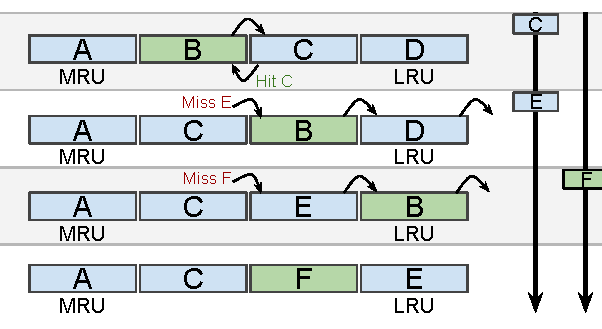
\includegraphics[width=.65\textwidth]{figures/algorithms/PIPP}
    \caption[PIPP managed 4-way cache set.]{PIPP managed 4-way cache set. (Two cores each allocated two blocks)}
    \label{fig:algorithms:pipp_example}
\end{figure}
\subsection{PriSM}
\label{sec:algorithms:prism}

\gls{prism}~\cite{Manikantan2012} was first presented in 2012.
\gls{prism} is a framework for cache management with optimization algorithms targetting multiple performance goals.
The original paper presents hit maximization, fairness and \gls{qos} goals.
We will focus on the hit maximization algorithm , or miss minimization algorithm, as all other algorithms in this thesis also targets this goal.
\gls{prism} utilizes \glspl{atd} to estimate private cache performance for each of the cores.
The \gls{atd} will keep track of total misses and hits.
It will not track hits per cache way like the \glspl{atd} in \gls{ucp} and \gls{pipp}.
In addition to the \glspl{atd}, the algorithm requires three counters per core tracking hits, misses and number of blocks owned by the core in the actual cache.
\gls{prism} utilizes the same insertion and promotion policies as \gls{lru}, but the replacement policy is optimized based on the \gls{atd} and the optimization target.

The replacement algorithm of \gls{prism} utilizes eviction probabilities, $E_i$ ($\sum{E_i} = 1$), assigned to each core when selecting a victim block.
On replacement, a victim core is first selected by a random draw using the eviction probabilities.
The \gls{lru} block owned by the victim core within the cache set is the eviction target.
In the case where the selected target does not own a block in the set, all blocks owned by cores with $E_i > 0$ are considered, and the \gls{lru} of these is the eviction target.
At set intervals, an optimization algorithm determines the eviction probability, $E_i$, for each core.
The original paper recalculated $E_i$ values at every 10000 cache miss.

The insertion and promotion policy of \gls{prism} is equal to \gls{lru}.
On insertion, a block is promoted to the \gls{mru} position, and on any subsequent accesses the block is again promoted to \gls{mru} unless it already has that position.

Selecting an eviction probability $E_i$ for each core is done by considering how the eviction probability will effect a core's usage of the cache.
Consider an interval of W misses where each core contributes a fraction of the misses, $M_i$.
At the start of the interval the blocks owned by $core_i$ equals a fraction $C_i$ of the total number of blocks in the cache.
If we do not evict any blocks owned by $core_i$ during the interval, then at the end of the interval the core owns a fraction $T_i$ of the cache.
$T_i$ is known as the target allocation, and is expressed by $T_i = C_i + M_i * W/N$. 
Here $M_i * W$ is the number of misses caused by $core_i$ during the interval, which also is the number of blocks inserted by the core.
$N$ is the total number of blocks in the cache, and the fraction $M_i * W/N$ equals the fraction of the cache claimed by $core_i$ during the interval.
If the core has a non-zero eviction probability, then this formula extends into $T_i = C_i + (M_i - E_i) * W/N$.
As noted, \gls{prism} defines three optimization targets, each one of these is responsible for calculating the optimal $T_i$ that will fulfill the optimization target.
Rearranging the above formula for $E_i$ yields: $E_i = (C_i - T_i) * N/W + M_i$.
Algorithm~\ref{alg:algorithms:prism} shows how $T_i$ values are calculated for hit maximization.
It is a relatively simple algorithm that will adjust the target occupancy based on the current occupancy and the potential for gaining more hits.

\begin{algorithm}[ht]
\caption{PriSM Hit Maximization.}
\label{alg:algorithms:prism}
\begin{algorithmic}[1]
\State $N$ /* Number of cores */
\ForAll{$cores\ i$}
    \State $PotentialGain[i]\gets StandAloneHits[i] - SharedHits[i]$
\EndFor
\State $TotalGain\gets \sum{PotentialGain}$

\ForAll{$cores\ i$}
    \State $T_i\gets C_i * (1 + \frac{PotentialGain[i]}{TotalGain})$
\EndFor
\State $T_i = \frac{T_i}{\sum{T}}$ /* Normalize target occupancy */
\end{algorithmic}
\end{algorithm}

While we have presented \gls{prism} based on \gls{lru} replacement, as done in the original paper, it should be noted that \gls{prism} is not dependent on this underlying replacement algorithm.
Any algorithm is usable, as long as it is augmented to prioritize the selected victim during replacement.
The algorithm run on the \glspl{atd} has to be the same as the underlying algorithm in the \gls{prism} implementation.

\section{CLU}
\label{sec:algorithms:clu}

CLU, short for Co-Optimizing Locality and Utility, is an algorithm presented by D. Zhan et al.~\cite{Zhan2014} in 2014.
The authors of CLU recognize that recent research in LLC partitioning has followed two distinct directions.
Some publications optimize for locality, and attempts to improve performance by chaning the lifetime of blocks in LRU managed caches.
DIP, TADIPm and NUCache are three such solutions that use novel methods to reduce or extend the lifetime of blocks in an elsewise LRU managed cache.
Other publications recognize the usefulness of utility and do way-prartitioning between cores based on their utility values.
Examples here are UCP and PIPP.
Because utility calculations are based on the stack property of LRU~\cite{Qureshi2006, Xie2009} both PIPP and LRU is unable to evaluate the utility of other algorithms that may violate this property.

The authors of CLU presents a novel approach for calculating the utility curve of a BIP managed cache.
BIP, as covered earlier, is one of the two insertion policies under DIP and TADIP. 
BIP violates the stack property of LRU by mostly inserting new rows at the MRU position, or at a low probability in LRU position.
In order to correctly measure the utility curve of a BIP managed k-way cache, one needs k ATDs; ATD(1), ATD(2), ... ATD(k). 
Where ATD(x) is an x-way ATD.
In contrast, the utility curve of an LRU managed cache can be found using one ATD, due to the stack property.
Having k ATDs per core sharing the LLC is not a realistic goal due to the required overhead.
The authors of CLU proposes a simplification where there are $m = log_2 k$ ATDs; ATD(1), ATD(2^1), ..., ATD(2^m).
A linear increase between the sample points is assumed when calculating the final utility curve.
It should be noted that the storage overhead of the m ATDs in total is less the twice the overhead of the single ATD(k) required to sample the LRU curve.

CLU uses the two curves to first allocate ways to each core using the same algorithm as shown for UCP in section~\ref{sec:algorithms:ucp}.
The only difference is that the algorithm uses either the LRU of BIP value when estimating utility given an allocation, depending on which algorithm performs best.
During runtime, CLU works like UCP, with the expectation that insertions are either done as in LRU or as in BIP, depending on which algorithm has the highest utility given the number of ways currently assigned to the respective core.
